\section{Model, Problem, and Related Works}
\label{sec:swapping_problem}

In this section, we discuss our network model, formulate the problem addressed, and discuss 
related work. 

\para{Network Model.} 
We denote a quantum network (QN) with a graph $G = (V, E)$,
with $V = \{v_1, v_2, \ldots, v_n\}$  and $E = \{(v_i, v_j)\}$
denoting the set of nodes and links respectively.
%%%%
Pairs of nodes connected by a link are defined as \textit{adjacent} nodes. 
%%%%%%%%%%%%%%%%%%
We follow the network model in~\cite{caleffi} closely.
%Fundamentally, each network node $A$ should be capable of generating atom-photon \epss, so that it can generate an atom-atom \epss with an adjacent node $B$.
%with the help of a 
%optical (photon-photon) BSM device situated exactly in between $A$ and $B$.
%%%%%%%%
Thus, each node has an atom-photon \eps generator with generation 
latency (\gt) and probability of success (\gp). Generation latency
is the time between successive attempts by the node to excite the 
atom to generate an atom-photon \eps; this implicitly includes the times for
photon transmission, optical-BSM latency, and classical acknowledgement.
\textit{For clarity of presentation} and without loss of generality,  
we assume homogeneous network nodes with same parameter values.
The generation rate is the inverse
of generation latency, as before.
A node's atom-photon generation capacity/rate 
is its aggregate capacity, and may be split across its incident links 
(i.e., in generation 
of \epss over its incident links/nodes).
Each node is also equipped with a certain number of atomic
memories to store the  qubits of the atom-atom \epss. 

\begin{figure}
%\begin{wrapfigure}{r}{2.1in}
    \centering
    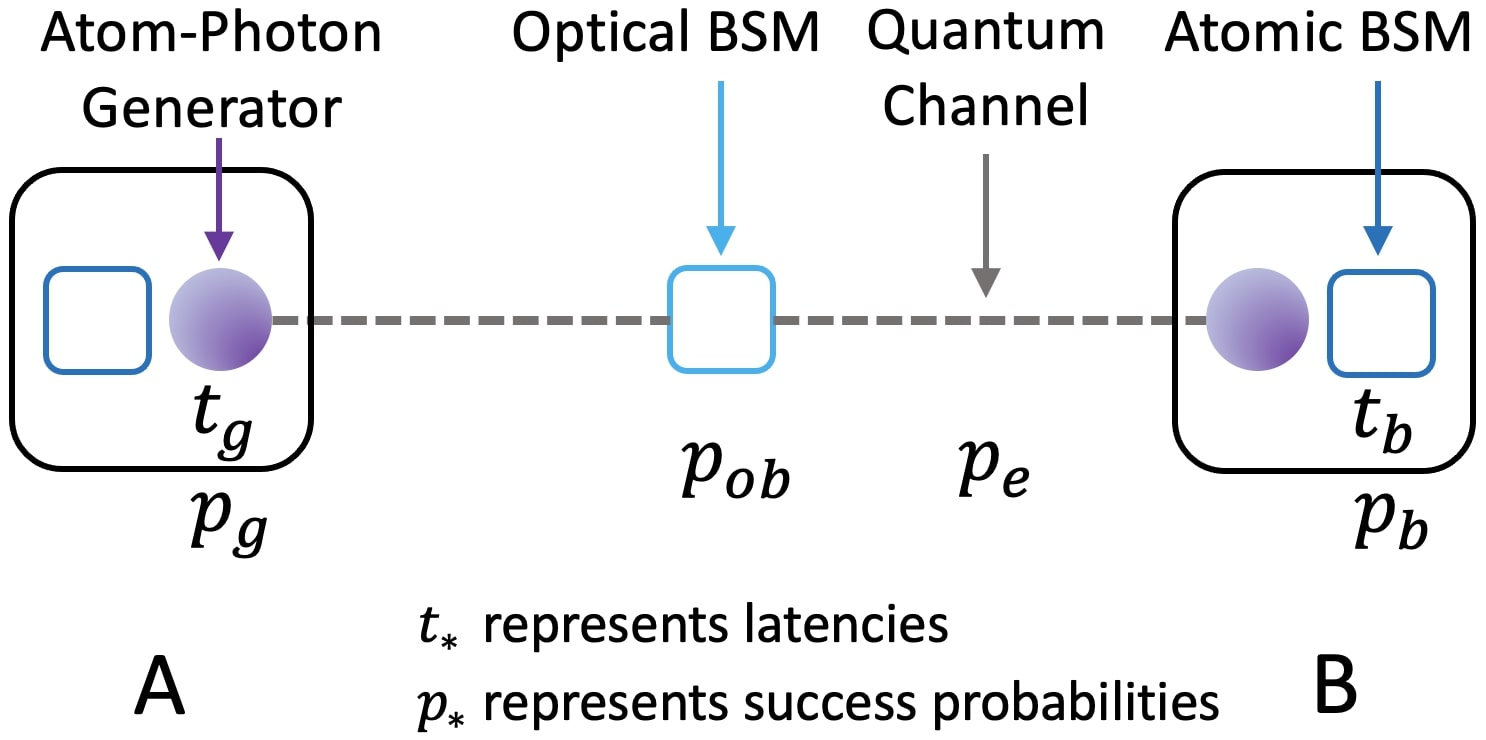
\includegraphics[width=0.65\textwidth]{chapters/swappingtrees/figures/notation_link.jpg}
  \vspace{0.3cm}
  \caption{Key notations used.}
  \label{fig:swapping_notation_link}
%\end{wrapfigure}
\end{figure}
A network link is a quantum channel (e.g., using an 
optical fiber or a free-space link),
and, in our context, is used only for establishment 
of link \eps.
%%%%%%%%%%%%%%%%%
In particular, a link $e=(A,B)$ is used to transmit telecom-photons 
from $A$ and $B$
to the photon-photon BSM device in the middle of $e$.
Thus, each link is composed of two 
half-links with a probability of transmission success (\ep) that decreases exponentially with the link distance (see~\S\ref{sec:swapping_eval}).
%and thus can be different for different links. 
The optical-BSM operation has 
a certain probability of success (\php).
%The above network aspects are sufficient to determine the maximum generation 
%rate of \epss over adjacent nodes (see below). 
To facilitate atom-atom \es operations, each network node is also equipped 
with an atomic-BSM device 
with an operation latency (\bt) and probability of success (\bp). Finally, 
there is an independent classical network with a transmission latency (\ct);
we assume classical transmission  
always succeeds.
%Classical transmission is used for acknowledgments, and in  teleportation and \es operations.

\softpara{Single vs.\ Multiple Links Between Nodes.}   For our techniques multiple links between a pair of  adjacent nodes can be replaced by a single link of aggregated
rate/capacity.  Hence we
assume only a single link between every pair of nodes. However, 
distinct multiple links between nodes have been used creatively
in~\cite{sigcomm20} (which refers to them as multiple channels); thus, we will 
discuss multiple links further in~\S\ref{sec:swapping_eval} when we evaluate various techniques. 
We note that the all-photonic protocol in~\cite{all-photo-15} is essentially a more sophisticated version of the multi-link \os protocol in~\cite{sigcomm20} to further
minimize memory requirements, but it uses multipartite cluster states which are
challenging to create. In either case, in terms of selection of paths/trees,
the path-selection techniques from~\cite{sigcomm20} should also apply to the all-photonic protocol with certain modifications to account for 
how the cluster states are generated.

%\subsection{Computing \eps Generation Latencies}
%%%% Caleffi does on-demand, i.e., excites the node's atom after the whole process fails or succeeds. Thus
%%%  he uses (total expected time)/probability of success.
%%%% IF the atom-photon EPS are being continuously generated anyway, then the rate is just that ... if we assume
%%%% photon/bsm are not overloaded. 


\eat{
\para{Link \eps Generation Latency.} 
Based on the above network model, the link \eps generation latency can be determined as follows. If a node is generating atom-photon \eps with a latency of \gt 
(i.e., at a rate of 1/\gt) with a probability of success of \gp, 
then the generation latency of a \textit{successful} atom-photon \eps is \gt/\gp 
and that of simultaneously generating two successful atom-photon \epss at a pair
of adjacent nodes is $\gt/\gp^2$. 
%Note that the atom-photon \eps generators across adjacent nodes are  perfectly synchronized, so that the photons reach the optical-BSM device at the same time.
%%%%%%%%%%%%%%%%
Since the success-probability of photon transmission and optical BSM 
processes are \ep and \php respectively, 
the overall latency of a successful \eps generation at a link is:
\begin{equation}
\frac{\gt}{\gp^2\ep^2\php} 
\label{eqn:swapping_link-rate}
\end{equation}
\eat{Above, we are implicitly assuming that 
the photon-transmission and 
BSM operation latencies 
are significantly lower than \gt/\gp~\cite{caleffi}.
else continuous 
generation of atom-photon \epss at nodes
will result in an overflow. (See Eqn.~\ref{eqn:swapping_gen-link-rate} 
for a more general expression.)}
The exact expression above has no bearing 
on the applicability or correctness of our techniques, 
but is presented largely for understanding of our model.
}
%%%%%%%%%%%%%
%%%is \bt and \bp respectively, the overall \eps link rate is: $$ \frac{1}{(1/(\gr\gp^2) + \et + \bt + \tc)/\bp)}$$
%%% Thus, the total time to generate an \eps over a link can be estimated by: $$1/(\gt\gp^2\ep^2\bp) + \et + \bt + \tc$$.


%A and B are two neighboring nodes that are connected by a quantum channel (classical channel omitted). Each node has an atom-photon generator and an atomic BSM device. There is an optical BSM device right in the middle of the quantum channel.}

\para{\eps Generation Latency of a Swapping Tree.} 
Given a swapping tree and \eps generation rates at the leaves (network links), we 
wish to estimate the generation latency of the \epss over the remote pair corresponding
to the tree's root with the \wt protocol. 
Below, we develop a recursive equation.
%%%%%%%%%%%%%
Consider a node $(A,C)$ in the tree, with $(A,B)$ and $(B,C)$ as its two children. 
Let $T_{AB}, T_{BC}$, and $T_{AC}$ be the corresponding (expected) generation latencies 
of the \epss over the three pairs of nodes. Below, we derive an expression for $T_{AC}$
in terms of  $T_{AB}$ and $T_{BC}$; this expression will be sufficient to determine the
expected latency of the overall swapping tree by applying the expression iteratively.
We start with an observation.
% \begin{observation}
If two \eps arrival processes $X_1$ and $X_2$ are exponentially distributed 
with a mean inter-arrival
latency of $\lambda$ each, then the expected inter-arrival latency of 
$\max(X,Y)$ is $(3/2)\lambda$.
\label{ob:swapping_expdist}
% \end{observation}
From above, if assume $T_{AB}$ and  $T_{BC}$ to be exponentially 
distributed  
with the same expected generation latency of $T$, 
then the expected latency of both \epss arriving is $(3/2)T$. 
Thus, we have: 
\begin{equation}
T_{AC} = (\frac{3}{2} T + \bt + \ct)/\bp, \label{eqn:swapping_tree-rate}
\end{equation}
%%%%%
\softpara{Remarks.}
We make the following remarks regarding the above expression.
%%%%%%%%%
First, when $T_{AB} \neq T_{BC}$, we are able to only derive an upper-bound on 
$T_{AC}$ which is given by the above equation but with $T$ replaced by
$\max(T_{AB}, T_{BC})$.\footnote{\tqbl{The 3-over-2 formula as an upper bound has also
been corroborated in a recent work~\cite{analytical22} which derives analytical bounds 
on \eps latency times in more general contexts.}}
% However, in our methods, the above assumption of $T_{AB} = 
% T_{BC}$ will hold as we would only be considering ``throttled'' trees to save on 
% underlying network resources (see~\S\ref{sec:swapping_single-path}).
\tqbl{Second, our motivation for the exponential distribution assumption stems from the
fact that the \eps generation latency at the {\em link level} is certainly exponentially
distributed if we assume the underlying probabilistic events to have a Poisson distribution.}
Third, note that
the resulting distribution is not exponential. 
Despite this, we apply the above equation recursively to compute the tree's generation
latency. 
% However, in our evaluations, we observe the validity of this approximation since our analysis matches closely with the simulation results. 
Finally, Eqn.~\ref{eqn:swapping_tree-rate}
% Eqn.~\ref{eqn:tree-rate} 
is conservative in the sense that 
each round of an \eps generation of any subtree's root starts from 
\tqbl{scratch (i.e., with no link \epss from prior round) }
and ends with either a 
\eps generation at the \textit{whole swapping tree}'s root
or an atomic-BSM failure at the subtree's root.
We do not ``pipeline'' any operations across rounds within a subtree, which may lower
%In other words, This
%implicitly discards link \epss while the previous round is in progress.
%Further enhancements of our protocol that doesn't discard \epss while carefully managing available memory may be able to achieve lower generation 
latency; this is beyond this work's scope. 

%%%%%%%%%%%%%
\eat{
Lastly, in the \os protocol, the expected generation 
latency is much higher due to the low-probability of \emph{all} 
of the underlying processes succeeding at the same time/time-slot. 
In addition, the \os protocol
requires that the underlying links be synchronized (which is not required
in the above \wt protocol). The expected generation latency in the \os protocol
is simply 
\begin{equation}
\frac{\gt}{(\gp^2\ep^2\php)^l\bp^l},  
\end{equation}
if we assume the link-\eps generation latency is uniformly \gt. Above, the path
length is $l$. When we have multiple links between adjacent nodes, then the expression
for generation latency is more complex as derived in~\cite{sigcomm20}.}


\subsection{Problem Formulation}
\label{sec:swapping_formulation}

We now formulate the central problem of selecting a \textit{single} swapping trees for a single source-destination pair. 

\para{\qnr Single Path (\spp) Problem.} Given a quantum network and a source-destination pair $(s,d)$, 
the \spp problem is to determine a single swapping tree that maximizes the expected
generation rate (i.e., minimizes the expected generation latency) of \epss over
$(s,d)$, under the following capacity and fidelity constraints:

% \para{Quantum Network Routing (\qnr) Problem.}
% Given a quantum network and a set of source-destination pairs $\{(s_i, d_i)\}$, 
% the \qnr problem is to determine a set $\T_i$ of swapping trees for each pair $(s_i, d_i)$ 
% such that the sum of the \eps rates 
% of all the trees in $\bigcup_i \T_i$ is maximized under the following 
% constraints: 
\begin{enumerate}
    \item \textit{Node Constraints.} For each node, the aggregate resources used by $\bigcup_i \T_i$ is less than the available resources; we formulate this formally below.
    \item \textit{Fidelity Constraints.} Each swapping tree in $\bigcup_i \T_i$ satisfies the following: (a) Number of leaves is less than a given threshold $\fidl$; this is to limit fidelity degradation due to gate operations. (b) Total memory storage time of any qubit is 
    less\footnote{\tqbl{We note that, in our context, the storage time as well as the memory coherence 
    time are statistical quantities due to the underlying statistical mechanisms. However, for the purposes of {\em selecting} a swapping tree, we use a fixed decoherence threshold \fidd\ value equal to the mean of the distribution of the coherence time (recent work~\cite{boxi-2020} computes optimal cut-offs/thresholds, and their techniques can be used to pick \fidd). When simulating a selected tree for generation of EPs, we can implement coherence time as a statistical measure.}}
    than a given \textit{decoherence threshold} $\fidd$.
\end{enumerate}
Informally, the swapping-trees may also satisfy some fairness constraint across the given 
source-destination pairs. A special case of the above \qnr problem is to select a single tree
for a source-destination pair; we address this in the next section. 

\softpara{Formulating Node Constraints.} 
Consider a swapping tree $\T \in \bigcup_i \T_i$  over a path $P$. For each link
$e \in P$, let $R(e, \T)$ be the \eps rate  being used by \T over the link $e$ in $P$. 
Let us define $R_e = \sum_\T  R(e,\T)$, and let $E(i)$ be the set of edges incident on $i$.
Then, the node capacity constraint is formulated as follows.
\begin{eqnarray}
1/\gt &\geq& \sum_{e \in E(i)} R_e/(\gp^2\ep^2\php) \ \ \ \  \forall i \in V. \label{eqn:swapping_qnr-1}
%1/\et &\geq& R_e/(\red{\gp}\ep^2\php)    \ \ \ \  \forall e \in E. \label{eqn:qnr-2}
\end{eqnarray}
\tqbl{The above comes from the fact that to generate a single link \eps over $e$, each end-node of $e$ needs
to generate $1/(\gp^2 \ep^2 \php)$ photons successfully, since each photon (from each end-node) 
has a generation success of \gp and a transmission success rate of \ep, and the optical-BSM's success
probability over the two successfully arriving photons is \php. Note that $1/\gt$ is a 
node's total generation capacity.}
Also, the memory constraint is that for any node $i$, the memory available in $i$ should be more than $2x + y$ where $x$ is the number of swapping trees that use $i$ as an intermediate node 
and $y$ is the number of trees that use $i$ as an end node. 



For homogeneous nodes and link parameters, it is easy to see that the best swapping-tree is the balanced or almost-balanced tree over the shortest path.
% We note that \spp is not a special case of \qnr in the formal sense; e.g., 
% the LP algorithm (\S\ref{sec:swapping_multiple-path}) for \qnr cannot be used for the \spp problem, due to the single tree requirement (LP may produce multiple trees).
As described in \S\ref{sec:swapping_related}, the \spp problem has been addressed before in~\cite{sigcomm20, caleffi} under different models. 
The problem of selecting \textit{multiple} swapping trees for \textit{multiple} source-destination pairs is solved in~\cite{tqe22-quantum}.




\subsection{Related Works}
\label{sec:swapping_related}

There have been a few works in the recent years that have addressed generating long-distance \epss
efficiently. All of these works have focused on selecting an efficient routing path for the swapping
process \bleu{(\cite{caleffi} also selects a path, but using a metric based
on balanced trees). }
In addition, all except~\cite{caleffi} have looked at the \os protocol of generating the
\epss. Recall that in the \os model, selection of paths suffice, while in the \wt model, one needs
to consider selection of efficient swapping trees with high fidelity.
%%%%%%%%%%%%%%%%%%%%%%%
Selection of optimal swapping trees is a fundamentally more challenging problem 
than selection of paths---and has not 
been addressed before, to the best of our knowledge. \eat{Efficient use of intermediate \epss rather than
discarding them (as in the \os protocol) has been mentioned as an open problem in~\cite{sigcomm20};
our paper addresses this challenge by using the \wt protocol.} We start with discussing how the \os model
works.

\para{\os Approaches.}
The most recent works to address the above problem are~\cite{sigcomm20} and~\cite{delft-lp}, 
both of which consider the \os model. 
In particular, Shi and Qian~\cite{sigcomm20} design a Dijkstra-like algorithm to construct an optimal path
between a pair of nodes, when there are multiple links (channels) between adjacent nodes. Then,
they use the algorithm iteratively to select multiple paths over multiple pairs of nodes.
%%%%%%%%%%
Chakraborty et al.~\cite{delft-lp} design a multi-commodity-flow
like LP formulation to select routing paths for a set of source destination pairs. They map
the operation-based fidelity constraint to the path length (as in~\cite{BreigelEtAl1998}), and use
node copies to model the constraint in the LP. However, they explicitly assume that the link
\eps generation is deterministic---i.e., always succeeds. 
%%%%%%%%%%%%%%%%%%%%%%%%%%%%%%%%%%%%%
Among earlier relevant works,~\cite{guha} proposes a greedy solution
for grid networks, and~\cite{greedy2019distributed} proposes 
virtual-path based routing in ring/grid networks.
\eat{and~\cite{gradient} using a gradient approach to select
efficient routing paths.}

\para{\wt Approach.}
Due to photon loss, establishing long-distance entanglement between remote
nodes at $L$ distance by \textit{direct} 
transmission yields \eps rates that decay exponentially with $L$. 
DLCZ protocol~\cite{dlcz,gisin} broke this exponential barrier using
$2^k$ equidistant intermediate nodes to perform entanglement-swapping operations, 
implicitly over a balanced binary tree, with a \wt protocol; this makes the 
\eps generation rate decay only polynomially in $L$. \eat{This is fundamental to the feasibility of establishing long-distance entanglements.}
%%%%%%%%%%%%
More recently, Caleffi~\cite{caleffi} formulated the entanglement generation rate on a given path between two nodes, under the more realistic condition where the intermediate nodes in the path may not all be equidistant, but still considered only balanced trees. Their path-based metric
%%%%%
was then used to select the optimal path by enumerating over the 
exponentially many paths in the network.

\begin{figure}
    \centering
    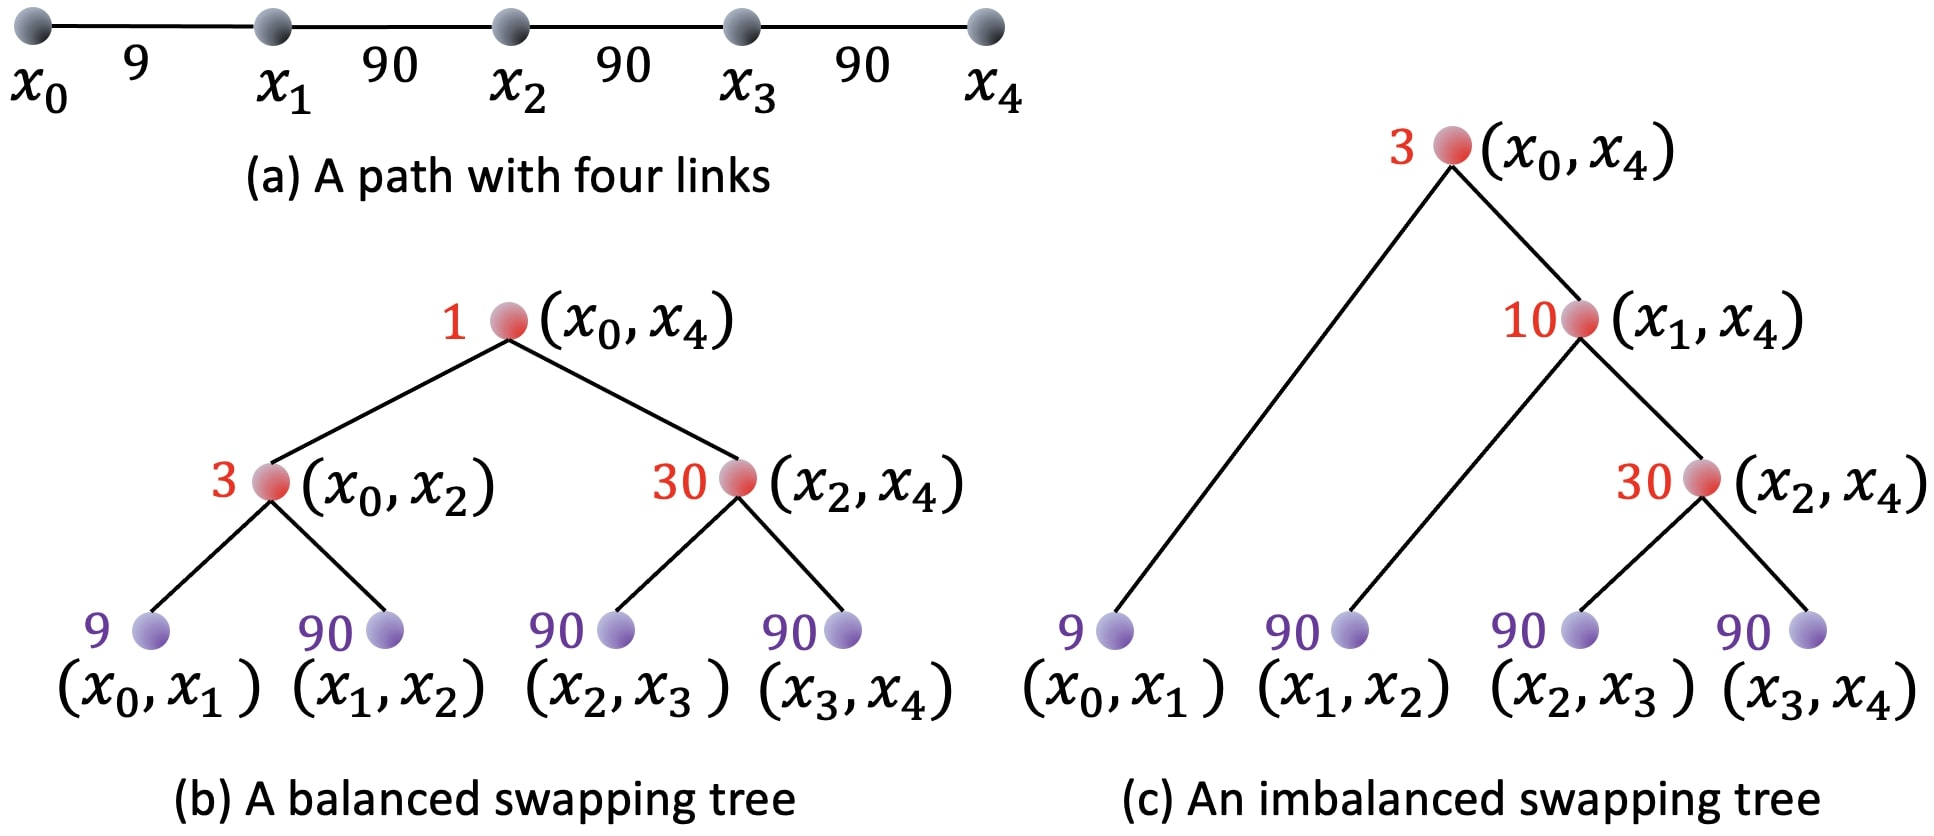
\includegraphics[width=0.75\textwidth]{chapters/swappingtrees/figures/non-balanced-balanced.jpg}
    % \vspace*{0.1in}
    \caption{Consider the path in (a). The imbalanced tree of (b) has a higher \eps generation rate than that of the balanced tree of (c). Here, the numbers represent the \eps generation rates over adjacent links or node-pairs.} 
    % \vspace*{-0.2in}
    \label{fig:swapping_non-balance}
\end{figure}


\softpara{Our Approach (vs.~\cite{caleffi}).}
Though~\cite{caleffi} considers only balanced trees, its 
brute-force algorithm is literally impossible to run for 
networks more than a few tens of nodes.
In our work, we observe that a path has many swapping trees, 
and, in general, imbalanced trees may even
be better; see Figure~\ref{fig:swapping_non-balance}. 
Thus, ~\cite{tqe22-quantum} design a polynomial-time dynamic programming (DP) algorithm that delivers 
an \textit{optimal} high-fidelity swapping-tree;
the approach effectively considers all possible swapping trees, 
not just balanced ones (note that, even over a single path, 
there are exponentially many trees). 
%Incorporation of fidelity (including decoherence) in our DP approach requires non-trivial observation and analysis (\S\ref{sec:swapping_dec}).
Our \dpalt Heuristic (\S\ref{sec:swapping_efficient}) is closer to~\cite{caleffi}'s work, 
in that both 
consider only balanced trees; however, we use a heuristic metric that facilitates a polynomial-time Dijkstra-like heuristic to select the optimal path, while their recursive metric~\footnote{We note that their formula (Eqn.~10 in~\cite{caleffi}) is incorrect as it either ignores the 3/2 factor or assumes the \eps generations to be synchronized {\bf across all} links. In addition, their expression for "qubit age" ignores the "waiting for \es" time completely. \label{ft:swapping_wrong}} 
(albeit more accurate than ours) is not amenable to an efficient (polynomial-time) search algorithm. 

\para{Other Works.}
In~\cite{Jiang17291}, Jiang et al.\ address a related problem; given a 
path with uniform link-lengths, they give an algorithm for selecting an 
optimal sequence of swapping and purification operations 
to produce an \eps with fidelity constraints.  
In other recent works, Dahlberg et al~\cite{sigcomm19} design physical and link layer protocols
of a quantum network stack, and~\cite{conext20} proposes a data plane protocol to generate \epss
within decoherence thresholds along a \emph{given} routing path. 
More recently, Bugalho et al.~\cite{bugalho2021distributing} propose an algorithm to efficiently distribute multipartite entanglement across over than two nodes.

\eat{
%%%%%%
Most recent works: sigcomm and delft-lp. They both do paths in \os model. 
\cite{sigcomm20} considers the \os model. For the \os model, if we assume a single channel per link, the \eps generation rate for a path (tree doesn't matter) can be
easily derived to be $p^n \bp^n$ per time slot. But, for multiple channels, it requires
a more complex metric -- derived in their paper.
%%%%%%
They use a Dijkstra like algorithm to find an optimal path. Use an iterative procedure
to find paths for more pairs. They use a simplistic model of resource -- multiple channels per link. }

\eat{

; this is clearly infeasible for even networks with 100’s of nodes. (?perhaps not needed?) 

\bleu{The \wt approach has been well analyzed in~\cite{gisin}; they implicitly consider
balanced trees over given paths. More recently,} Caleffi~\cite{caleffi} 
derives an expression\footnote{We note that their formula (Eqn.~10 in~\cite{caleffi}) is incorrect as it either ignores the 3/2 factor, or assumes the \eps generations to be synchronized {\bf across all} links. In addition, their expression for "qubit age" ignores the "waiting for \es" time completely. \label{ft:wrong}} for generation latency of a \textit{balanced} swapping 
tree over a path, and designs
a \bleu{brute-force \textit{exponential}-time algorithm to select an optimal path (by considering all possible simple routes and picking the one with lowest generation latency of the balanced tree).}
}

\eat{
Our dynamic programming approach is very different from~\cite{caleffi};
in effect,~\cite{caleffi} does exhaustive search of all paths, while
our dynamic-programming algorithm (\S\ref{sec:swapping_dp}) effectively considers 
all swapping trees (exponentially many, even
over a single path). 




\eat{Optimality of our approach rests on a non-trivial claim of ensuring disjoint subtrees (Lemma~\ref{lemma:swapping_subtrees}).
%%%%%%%%%%%%%%%%%%%%%%%%%
Incorporating fidelity and decoherence in~\cite{caleffi} is quite straightforward
(though,~\cite{caleffi} incorporates only decoherence; see Footnote~\ref{ft:swapping_wrong});} in contrast, in our dynamic programming approach, incorporation of fidelity (including decoherence) requires non-trivial observation and analysis (\S\ref{sec:swapping_dec}).
%%%%%%%%%%%%%%%%%%%%%
%%%%%%%%%%%%%%%%%%%%%%
Our \dpalt Heuristic (\S\ref{sec:swapping_efficient}) is closer to~\cite{caleffi}'s work, in that both 
consider only balanced trees; however, we use heuristic metric that facilitates a polynomial-time Dijkstra-like heuristic to select the optimal path, while their recursive metric (albeit more accurate
than ours) is not amenable to an efficient (polynomial-time) search algorithm. 
\cb
}


%We build upon it.
%Our work falls into developing a control plane protocol (routing) of the network layer for the quantum network stack.}


